\documentclass[11pt]{article}
\usepackage[margin=0.85in]{geometry}
\usepackage[T1]{fontenc}
\usepackage{lmodern,amsmath,booktabs,graphicx,microtype,float}
\usepackage[hidelinks]{hyperref}
\title{Experiments with $C_0=70$ and $L_0=16$\\Natural Empirical and Constructed Distributions}
\author{OSST project experimental artifact}
\date{22 October 2026}
\begin{document}\maketitle
\begin{abstract}
We execute the real-mean $(70,16)$ support-size construction on 756 constructed,
236 natural empirical, and 120 empirically shaped synthetic configurations.
The primary method is evaluated 4,208,000 times, including 1,672,000 actual
polynomial-branch trials. No promised binary error or support-bound failure
is observed. However, the same-budget count ablation also has no binary errors,
and a 99\%-guaranteed count baseline uses 2.44--8.39 times fewer expected samples
on the synthetic grid. Polynomial corrections improve 554,000 lower bounds.
We preserve negative comparisons, finite-file failures and dependence stress.
\end{abstract}
\section{Protocol and statistical scope}
We implement the construction in Qisheng Wang's \emph{Optimal Support Size Testing}
(supplied manuscript \texttt{2610.18723v1}) with the project's certified constants.
The algorithm uses $L=1+\ln n$, real Poisson mean
$m=70n/(\epsilon L)$, and the unchanged polynomial construction when $L\ge16$.
Its first integer polynomial input is $n=3,269,018$. We retain all scales,
degrees, corrections and decision thresholds; the largest tested degree is 162.
The supplied theorem gives individual failure below 0.282612 for the binary
promise problem and for support-bound coverage. $\epsilon$ is the distribution
separation parameter, not the failure probability.

Synthetic sizes range from 1 to $10^{12}$ and include three consecutive
integers at the branch boundary. Four epsilons are 0.001, 0.01, 0.1 and 0.25.
Uniform, concentrated-head, sparse-tail, power, lognormal, Gaussian-block,
geometric-block, boundary and gap distributions are included. Natural data add
$\epsilon=0.05$. Each primary synthetic/natural cell has four independent blocks
of 1000 trials; lifted-shape cells have four blocks of 500. Exact rational
tail masses determine promise labels. Gap inputs have no binary error label.
Code/data hashes were frozen before primary simulation, with no error-dependent
stopping. Different budgets use independent streams; same-budget ablations
share fingerprints. Method evaluations are not all independent samples.

\begin{table}[H]\centering\small
\begin{tabular}{lrrrr}\toprule
Suite & Cells & Outputs & Errors & Worst 95\% bound\\\midrule
Synthetic & 756 & 3,024,000 & 0 & 0.2817\% \\
Natural empirical & 236 & 944,000 & 0 & 0.2441\% \\
Lifted (synthetic) & 120 & 240,000 & 0 & 0.4660\% \\
27 independent runs & 50 & 50,000 & 0 & 0.7848\% \\
\bottomrule\end{tabular}
\caption{Primary method or amplified outputs. The last column is a percentage:
the worst cell's one-sided Clopper--Pearson upper bound with Bonferroni
correction across all non-gap method cells in its suite. Zero observed errors
do not establish zero risk. Support-bound coverage is checked separately.}
\end{table}
\begin{figure}[H]\centering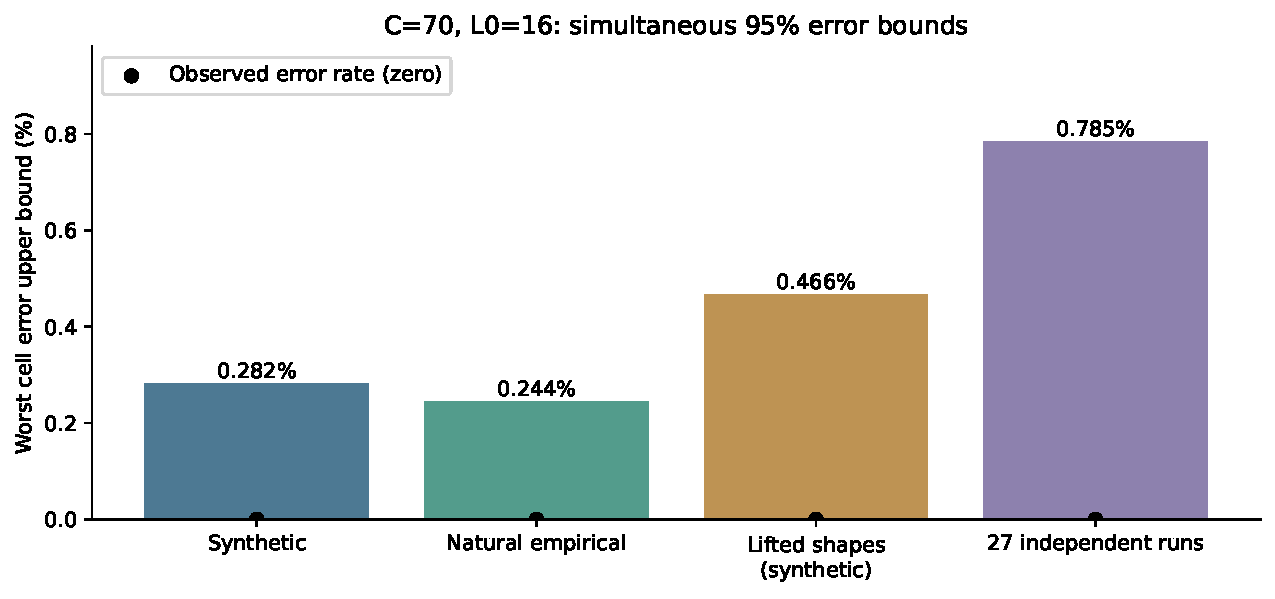
\includegraphics[width=.97\linewidth]{figures/risk.pdf}
\caption{Simultaneous error bounds, including the separate amplification experiment.}\end{figure}

\section{Samples, lower bounds and confidence}
Single-run samples are about 14.64 times fewer than for $(1025,1024)$,
but the uniform single-run confidence guarantees differ. At the same theoretical
confidence target, a certified count baseline still uses 2.44--16.30 times fewer
samples. Even the 99\% count baseline uses 2.44--8.39 times fewer samples.
This practical grid has $70/(1+\ln n)\ge2.44$, so the count statistic already
receives a substantial budget. The polynomial changes improve lower bounds,
not binary rejection counts, on this grid.

On the rare-tail null with $n=10^{12}$, $\epsilon=0.1$ and tail mass
$0.1\epsilon$, the mean observed fraction is about 0.2169 while the new lower
bound is about $0.5786n$. Here the effective support is only one; this illustrates
extra information, not recovery from a failed effective-support guarantee.

Using only $(70,16)$, 27 independent repetitions, majority voting and median
aggregation give per-task failure at most 0.008175637833. The expected total
coefficient is 1890, about 1.844 times the older coefficient 1025. A union bound
for either output failing is 0.016351275666, so we do not claim simultaneous
99\% correctness for both outputs. Fifty configurations each use 1000 aggregated
trials. The earlier $(70,20)$ results are not mixed into this experiment.
\begin{figure}[H]\centering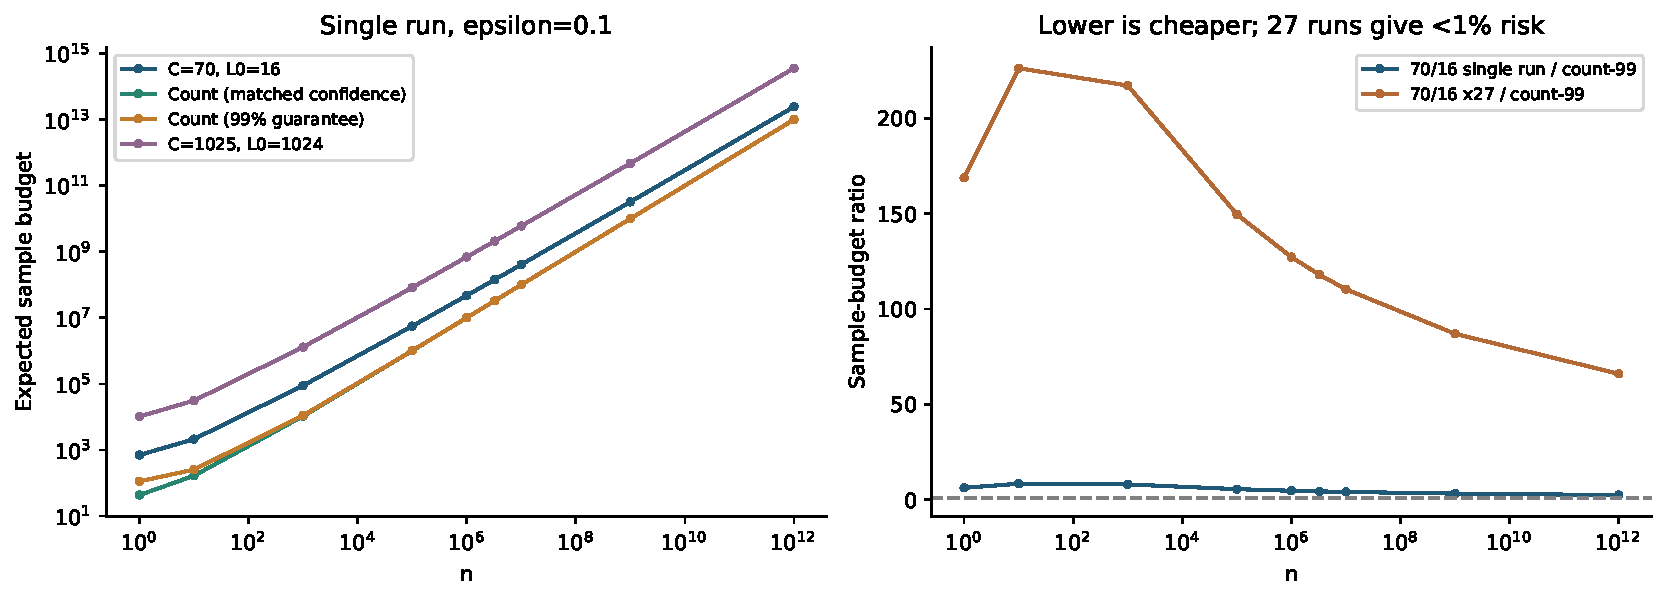
\includegraphics[width=\linewidth]{figures/budgets.pdf}
\caption{Expected sample costs and confidence-aligned repeated-run comparisons.}\end{figure}
\begin{figure}[H]\centering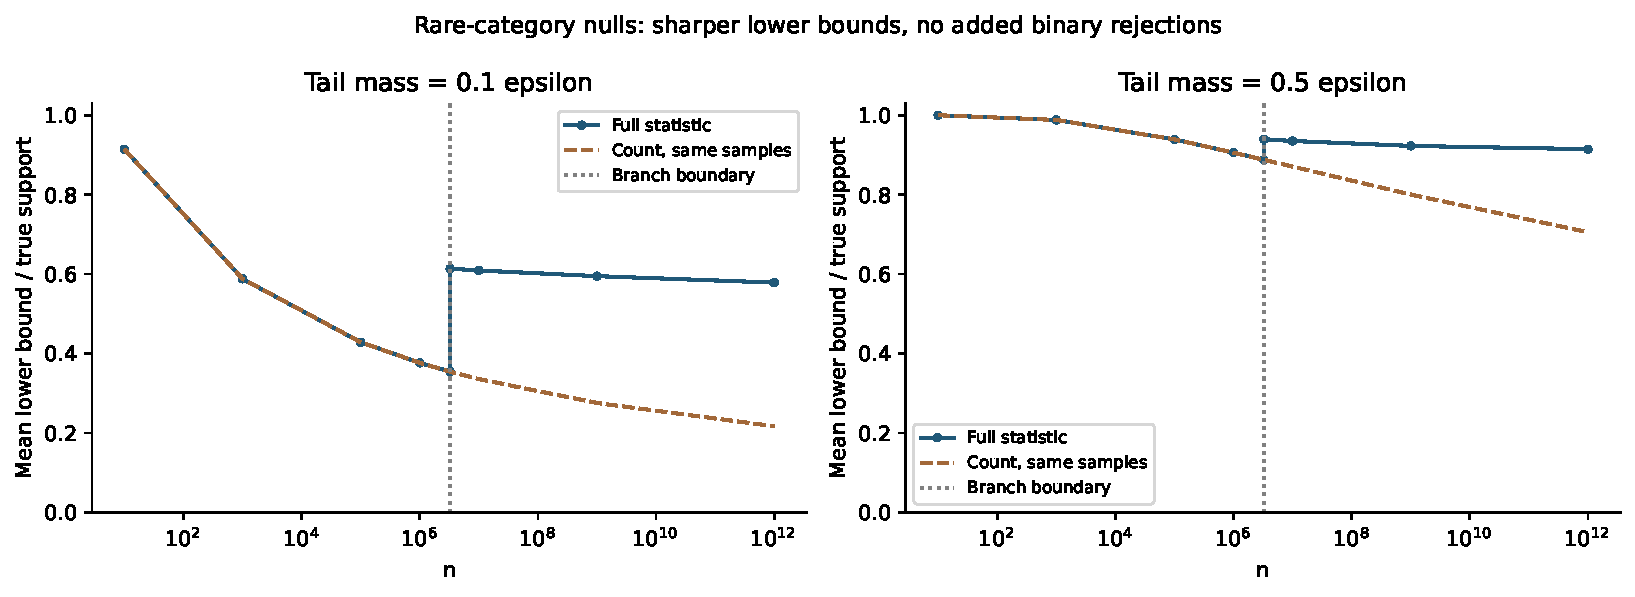
\includegraphics[width=\linewidth]{figures/lower_bounds.pdf}
\caption{Sharper lower bounds on rare-category nulls. The branch change is prescribed.}\end{figure}

\section{Natural data and dependence}
Ten finite empirical populations cover mites, birds at two sites, spiders under
two treatments, moths, land snails, BCI trees and fish from two year/gear strata.
Sources, pinned versions, hashes and licenses are retained in
\texttt{data\_sources.json}. No different years/sites/treatments are pooled.
All original natural populations use the count branch. Splitting each observed
category into equally probable synthetic clones creates separate lifted-shape
tests around $10^7$ and $10^9$ support; these are explicitly synthetic, not new
species observations. There are 116 polynomial lifted-shape configurations.

Only 42 of 236 natural configurations have enough original records to reach the
mean budget. Fixed-file tests retain every Poisson overflow as Inconclusive,
never truncate or resample until success. Successful without-replacement
subsamples are descriptive and do not establish unconditional iid risk for an
unknown ecosystem. Group holdouts and whole-group compound-Poisson resampling
are separate stress tests. Artificially duplicated observations produce failure
rates up to 100\%, despite preserving marginal labels and expected record count.
\begin{figure}[H]\centering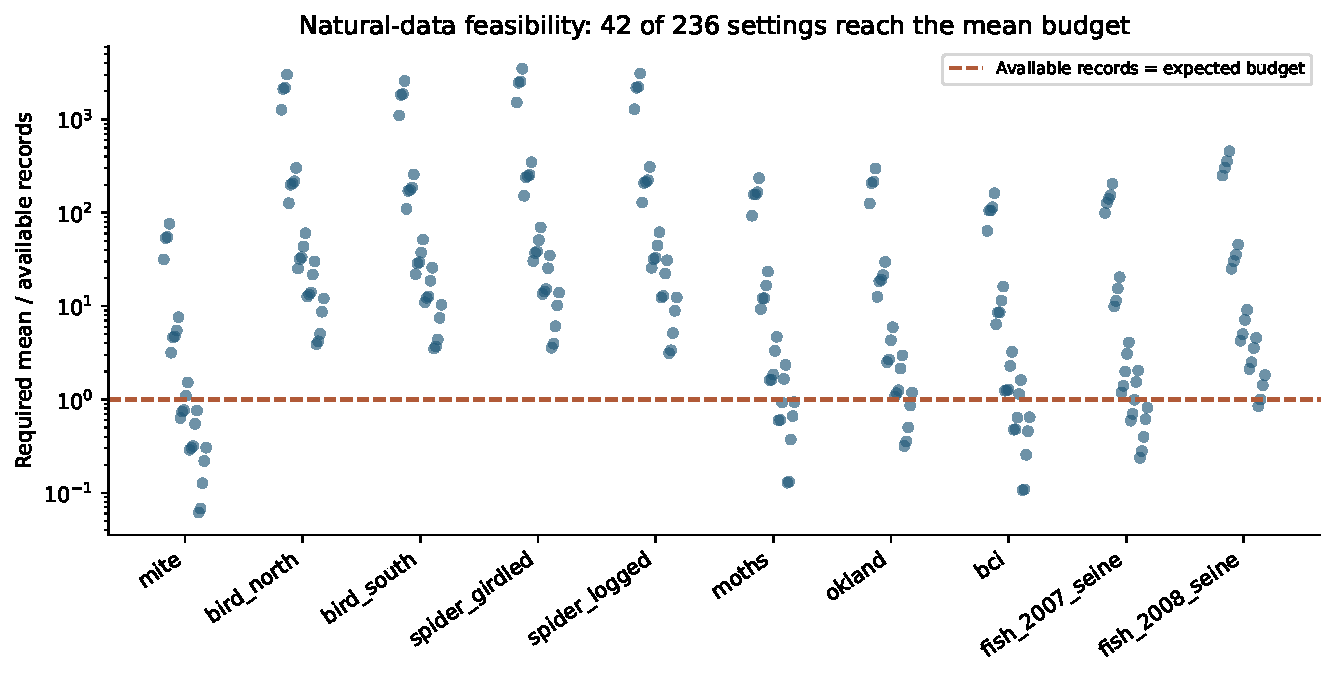
\includegraphics[width=.96\linewidth]{figures/natural_feasibility.pdf}
\caption{Original record budgets across natural configurations.}\end{figure}
\begin{figure}[H]\centering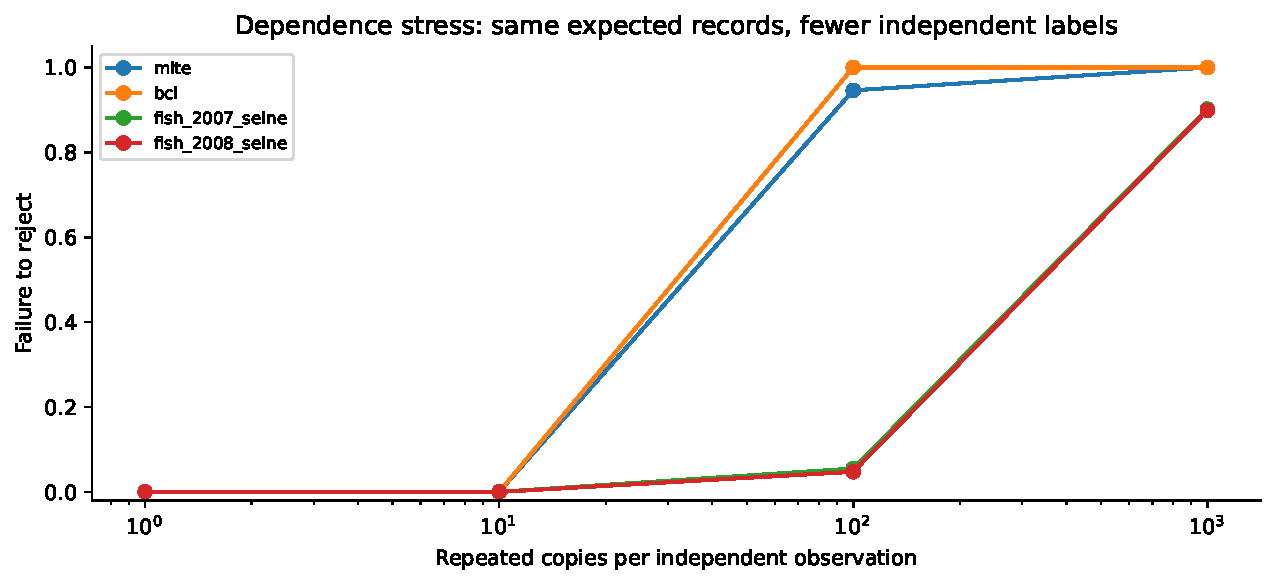
\includegraphics[width=.95\linewidth]{figures/dependence.pdf}
\caption{Artificial dependence invalidates the independent-sampling hypothesis.}\end{figure}

\section{Numerical validation and reproducibility}
Arb certifies real-mean parameters and full polynomial weights. Batched dot
products use outward enclosures and conservative IEEE-754 roundoff bounds;
unresolved event thresholds are refined with Arb. Every binary decision and
coverage event is certified on its supplied counts. Some exact integer lower
outputs remain enclosed in intervals; their means are reported as intervals,
not guessed integers. The public single-fingerprint interface increases
precision until it certifies the exact integer output or raises an error.

There are 8896 full-Arb primary checks, 476 further saved-profile checks at
1024 bits, and 18 explicit full-fingerprint API runs (12 polynomial). All
125 regression tests pass. The analytic proof's 428 exact obligations and
2491 independent arithmetic checks are recomputed with byte-identical results.
The final audit includes 113,951 checks.
This is not an end-to-end proof-assistant formalization.

Grouped multinomial fingerprints have the same law as independent Poisson
category counts in real arithmetic. Probability evaluation and pseudorandom
generation remain binary64 approximations. The high-count bucket retains
category counts without fabricating total observations $M$. No compressed
simulation timing is represented as physical sample-acquisition time.
\begin{figure}[H]\centering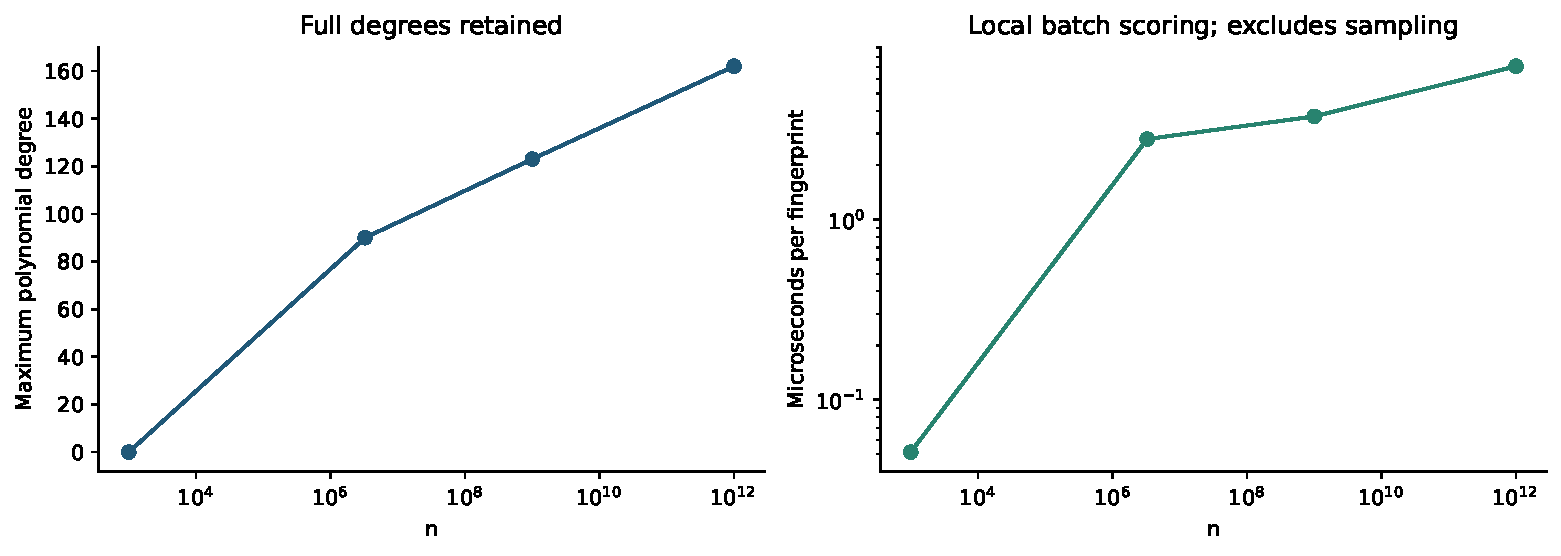
\includegraphics[width=\linewidth]{figures/runtime.pdf}
\caption{Full degree and local scoring cost, excluding physical data collection.}\end{figure}

\paragraph{Artifact.} Start with the Chinese \texttt{report.html}, then
\texttt{REPRODUCE.txt}, \texttt{protocol.json}, CSV summaries, exact population
specifications in \texttt{cells/}, and per-trial fingerprints in \texttt{raw/}.
The source snapshot and final manifest permit independent reruns. Statistical
success on this finite grid does not prove globally minimal constants, improved
asymptotic complexity, ecosystem completeness or a venue-acceptance claim.
\end{document}
